\section{RPM Measurement}
Real-time angular velocity measurement involves counting commutation signals transmitted via
an auxiliary cable from the ESC. This is achieved by utilizing an interrupt
trigger to record the time elapsed since the previous commutation in an array,
which resets after a defined sampling period. This approach enhances measurement
resolution compared to counting commutations within a specific sampling period.
Let $\hat \omega_{\delta t}$ represent angular velocity measured using commutation durations
($\delta t$) and $\hat \omega_{n_C}$ denote angular velocity measured using commutation
counts ($\delta n_C$) within a sampling period \cite{PX4-autopilot-rpm}.
%===
\begin{align}
    \hat \omega_{n_C} &= \frac{2 \pi n_C}{N_p f_s} \, rad/s, \quad
    \hat \omega_{\delta t} = \frac{2 \pi}{N_p  \delta t} \, rad/s
\end{align}
Where,
\begin{align*}
    N_p &- \text{No. of pole pairs in the motor (here, 7)}\\
    f_s &- \text{Sampling frequency}\\
    \delta t &- \text{Durtion between two commutations}\\
    n_C &- \text{No. of commutations within a sampling period}
\end{align*}
%===
In both cases, the minimum angular velocity from which the measurement begins is $\omega_{min} = \frac{2 \pi}{N_p f_s}$. This is because no commutation would be registered at a speed slower than $\omega_{min}$.

Commutation duration, denoted as $\delta t$, is determined by a higher frequency counter, $f_t$, which is not bound by the overall system sampling rate. Therefore, we can express $\delta t$ as $\delta t_k / f_t$.

As for the resolution of our measurement processes:
%===
\begin{align}
    &\abs{\Delta \hat \omega_{n_C}} = \frac{2 \pi \abs{\Delta n_C} }{N_p f_s} \\
    &\implies \abs{\Delta \hat \omega_{n_C}}_{\min} =\frac{2 \pi}{N_p f_s} = \omega_{min}\\
    %===
    &\abs{\Delta\hat \omega_{\delta t}} = \frac{2 \pi \abs{\Delta \delta t}}{N_p  \delta t^2} = \frac{\abs{\Delta \delta t}}{\delta t} \hat \omega_{\delta t} = \frac{\abs{\Delta \delta t_k}}{\delta t_k} \hat \omega_{\delta t}\\
    &\implies  \abs{\Delta\hat \omega_{\delta t}}_{\min} = \frac{\abs{\Delta \delta t_k}_{\min}}{\delta t_k} \hat \omega_{\delta t} = \frac{\hat \omega_{\delta t}}{\delta t_k}
\end{align}
%===
In this setup, the resolution of $\hat \omega_{n_C}$ remains constant at $\omega_{\min}$. However, in the case of $\hat \omega_{\delta t}$, the resolution depends on the instantaneous $\omega_{\delta t}$ and the frequency of the counter, $f_t$. Using a sufficiently fast counter ensures that the $\hat \omega_{\delta t}$ measurement process achieves significantly higher resolution compared to $\hat \omega_{n_C}$.

Given that multiple measurements of $\delta t$ occur within a single sampling
instance and that the process is susceptible to noise due to interrupt skips, we
adopt a median-based approach to estimate angular velocity at the end of a given
sampling
instance. Unlike other averaging methods, using the median effectively
eliminates spikes in $\delta t$ that can occur when an interrupt is skipped.
Detailed pseudocode for this algorithm is presented in Algorithm-\ref{alg::ISR}
and Algorithm-\ref{alg::get_rpm}.

%===

\RestyleAlgo{boxruled}
\LinesNumbered
\begin{algorithm}[H]
    \scriptsize
    $n_C \peq 1$\;
    \Comment*[l]{$C_c$ - Counter value at current interrupt}
    \Comment*[l]{$P_c$ - Counter value at previous interrupt}
    $\delta t_k = C_c - P_c$\;
    \If{ $\delta t_k \leq 0$ }
        {\Comment*[l]{Correcting for integer overflow}
         $\delta t_k \peq 2^{32}$}
    $\pmb{\delta t_k} [n_C-1] =  \delta t_k$\;
    $P_c = C_c$
    \caption{\small Interrupt Service Routine}
    \label{alg::ISR}
\end{algorithm}

%===
\RestyleAlgo{boxruled}
\LinesNumbered
\begin{algorithm}[H]
    \scriptsize
    $N_p = 7$\;
    $f_t = 10^6$\;
    $M = \frac{2 \pi}{N_p} \times f_t$\;
    \eIf {$n_C > 0$ and $n_C \leq n_{C_{max}}$ and $\norm{n_C - n_{C_{old}}} \leq \delta n_{C_{max}}$}
        {\Comment*[l]{Median removes spikes in the data}
         $\omega = \frac{M}{\text{Median}(\pmb{\delta t_k})}$\;
         $ \omega_{old} = \omega$\;
         $n_{C_{old}} = n_C$\;
        }
         {$\omega = \omega_{old}$}
    $n_C = 0$
    $\pmb{\delta t_k} = \pmb 0$\;
    \caption{\small RPM Measurement Function}
    \label{alg::get_rpm}
\end{algorithm}

%===
\begin{figure}[H]
    \centering
    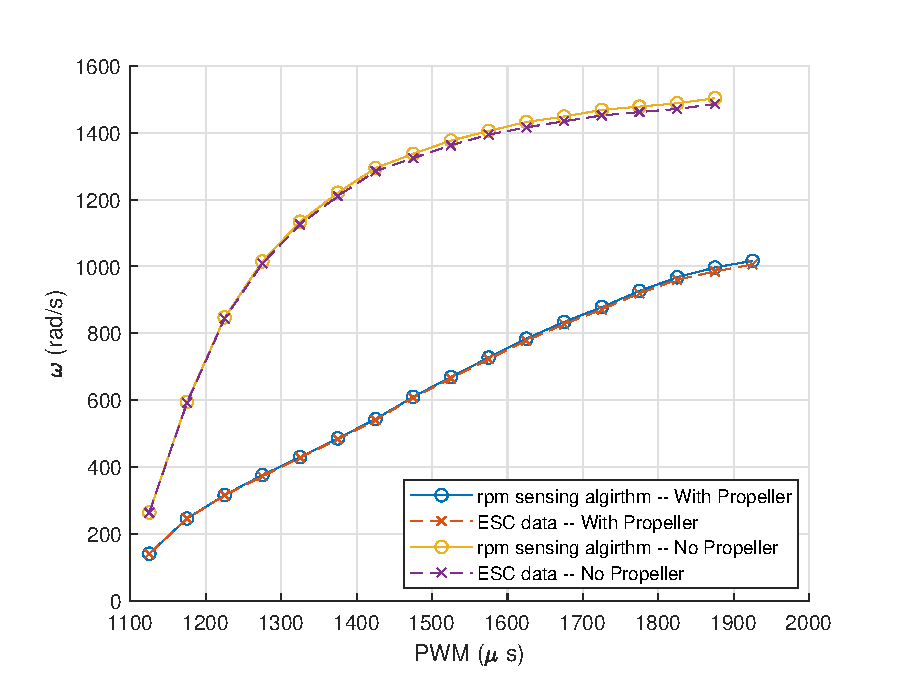
\includegraphics[width = \figsize]{./figs/figs_acc/rpm_feedback/rpm_meas.eps}
    \caption{RPM vs PWM with and without propeller}
    \label{fig::valid}
\end{figure}
%===
The measurement algorithm's validation process is conducted by comparing its results against the ESC data-log, as depicted in Fig.-\ref{fig::valid}. These validation plots not only confirm the algorithm's accuracy but also reveal the presence of non-linear input compensation mechanisms within the ESC.
